\begin{figure}
	\centering

	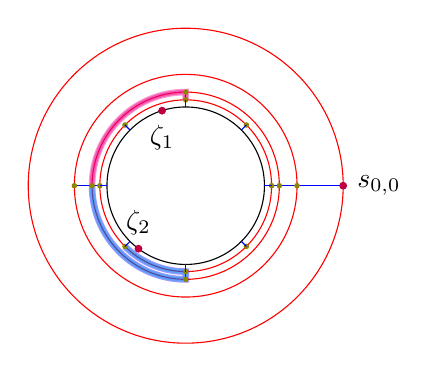
\begin{tikzpicture}
		
		
		\draw (0,0) circle (1);
		\draw[red] (0,0) circle (2);
		\draw[red] (0,0) circle (2^0.5);
		\draw[red] (0,0) circle (2^0.25);
		\draw[red] (0,0) circle (2^0.125);
		
		
		\draw [magenta,-, double=magenta, double distance=4\pgflinewidth, opacity=0.4,
		] (-1.189,0) arc (180:90:1.189) -- (0,1.0905);
		
		\draw [blue,-, double=cyan, double distance=4\pgflinewidth, opacity=0.4,
] (-1.189,0) arc (-180:-90:1.189) -- (0,-1.0905) arc (-90:-135:1.0905);
		
		\draw[blue] (2,0);
		
		\draw[blue] (2,0) --  (1,0);	
		\draw[blue] (-2^0.5,0) -- (-1,0);	
		\draw[blue] (0, 2^0.25) -- (0,1);	
		\draw[blue] (0, -2^0.25) -- (0,-1);	
		
		\fill[olive] (2,0) circle (1pt);
		\fill[olive] (2^0.5,0) circle (1pt);
		\fill[olive] (-2^0.5,0) circle (1pt);
		
		\foreach \angle in {0,90,180,270}
		\fill[olive] (\angle:2^0.25) circle (1pt);
		
		\foreach \angle in {0,45,90,135,180,225,270,315}
		\fill[olive] (\angle:2^0.125) circle (1pt);
		\foreach \angle in {0,45,90,135,180,225,270,315}
		\draw[blue] (\angle:2^0.125) -- (\angle:1);
		
		\node[circle,inner sep=1pt,fill=purple,label=below:{$\zeta_1$}] at (-0.3,0.953) {};

		\node[circle,inner sep=1pt,fill=purple,label=above:{$\zeta_2$}] at (-0.6,-0.8) {};
		
		\node[circle,inner sep=1pt,fill=purple,label={ right:{$s_{0,0}$}} ] at (2,0) {};
	\end{tikzpicture}

\caption{A quasiconvexity certificate between two points $\zeta_1,\zeta_2$.} \label{fig:Carleson2}
\end{figure}

